\chapter{Úvod}
Neuronové sítě (anglicky neural networks) mají v dnešním světě mnoho využití. Jelikož se jedná o jednu z aplikací umělé inteligence (anglicky artificial intelligence), lze neuronové sítě použít například k rozpoznávání řeči, zpracování přirozeného jazyka či k detekci objektů.
Tyto akce jsou pro běžného člověka poměrně snadné, avšak pro počítače znamenají relativně náročnou činnost.

Aby byly počítače schopné tyto akce vykonávat v rozumném čase (případně v reálném čase), je potřeba aby neuronové sítě byly dostatečně rychlé. Tato práce se zabývá akcelerací neuronových sítí v oblasti detekce obličeje. Zrychlení neuronové sítě lze dosáhnout buď optimalizací kódu, lepším trénováním neuronové sítě nebo také využitím speciálních hardwarových zařízení. Jedním z těchto specializovaných zařízení je Intel Neural Compute Stick 2, na něž se v této práci zaměřím. 

Následující kapitola se obecně věnuje problematice detekce obličeje v reálných podmínkách s využitím neuronových sítí. Je zde detailně popsáno \todo{CO JE DETAILNě Popsáno?}.

V kapitole \ref{kapitola:navrh_reseni} je nastíněn návrh akcelerace neuronové sítě pro detekci obličeje. \todo{\blindtext}

Kapitola \ref{kapitola:implementace} se věnuje implementaci programu ke zrychlení detekce, také obsahuje informace o využitých prostředcích.

Předposlední kapitola (kapitola č.\ref{kapitola:porovnani_vykonnosti}) poskytuje přehled experimentů a testů provedených s implementovaným řešením a s řešeními již existujícími. Hlavním tématem v této části je porovnání výkonnosti a zobrazení dosažených výsledků.

\nocite{*}
%%%%%%%%%%%%%%%%%%%%%%%%%%%%%%%%%%%%%%%%%%%%%%%%%%%%%%%%%
%       KAPITOLA 2
%%%%%%%%%%%%%%%%%%%%%%%%%%%%%%%%%%%%%%%%%%%%%%%%%%%%%%%%%

\chapter{Kamery a systémy pro detekci obličejů}
\label{kapitola:kamery_a_systemy}
Detekci obličejů s využitím počítačových programů lze provádět nad snímkem 
(fotografií, obrázkem), sadou snímků,
videozáznamem nebo tzv. real\,--\,timově pomocí kamer a kamerových systémů.
V této kapitole jsou popsány aktuálně využívané prostředky pro vytváření 
podkladů k detekci obličejů (kamery) a také dostupná řešení zabývající se 
detekcí, a to jak placené komerční, tak neplacené open-source systémy.

\section{Kamery}
Nezbytnou součástí oboru detekce obličejů jsou kamery a kamerové systémy.
Existují kamery specializované k detekci či rozpoznávání obličejů 
a kamery obyčejné, které pouze zprostředkovávají obraz dále ke zpracování.

Specializované kamery se používají například k zabezpečení objektů nebo
jako domovní videozvonky, kdy kamera (respektive její software) v zachyceném
obraze detekuje a rozpozná obličej, a následně může vykonat přiřazenou akci 
(spustit alarm, poslat notifikaci, umožnit osobě vstup...) \cite{securityCamsWeb}.

Další oblastí, kde se kamery s detekcí a rozpoznáváním obličejů uplatní je
bezesporu dohled ve veřejných prostorech (anglicky CCTV surveillance). 
Detekce obličeje může sloužit k hledání podezřelých osob v záznamech z dohledových
kamer. Tyto záznamy jsou shromážďovány na serveru, pomocí detekce jsou
z obrazu vyřezány fragmenty s obličeji lidí a poté jsou tyto fragmenty
porovnány rozpoznávacím algoritmem s obličeji hledaných osob. Při shodě
dochází k informování administrátora systému, který podnikne další kroky 
\cite{suspectIdentification}. 

Kamery tedy mají v doméně detekce obličejů nezastupitelnou roli, na 
jejich praktické využití v systémech a řešení pro detekci se zaměřuje následujících
podkapitola.

\section{Dostupná řešení}
Řešení umožňující detekci (a často i rekognici) obličejů lze rozdělit do dvou kategorií: 
komerční (placené, profesionální) a nekomerční (zdarma, open-source, amatérské).
V následujících dvou podkapitolách jsou popsány konkrétní systémy poskytující
detekci obličejů s jejich výhodami a nevýhodami.

\subsection*{Komerční}
Komerčně využívaná zařízení pro detekci, případně rekognici lze běžně zakoupit 
a používat ve firemním nebo domácím prostředí. Mezi zástupce těchto zařízení
patří například produkty firem Netatmo, Google, Nest \cite{securityCamsWeb2}.

\begin{figure}[H]
  \begin{center}
      \scalebox{0.5}{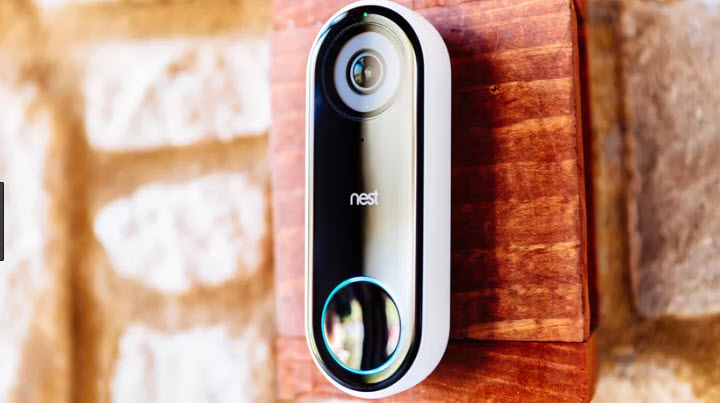
\includegraphics{obrazky-figures/nest-hello.png}}
  \label{nest}
  \caption{Nest Hello \cite{securityCamsWeb2}}
  \end{center}
\end{figure}

\subsection*{Nekomerční}
Nekomerční řešení pro detekci obličejů zahrnují frameworky s otevřeným zdrojovým
kódem (open-source). Tyto frameworky využívají neuronové sítě, které jsou trénovány
pomocí datasetů a následně je framework využit k detekci obličeje 
\cite{faceRecognitionFrameworks}.
Frameworky TinaFace \cite{TinaFace} a MTCNN \cite{MTCNN} mají zdrojové kódy
volně dostupné na webu GitHub.com.





%%%%%%%%%%%%%%%%%%%%%%%%%%%%%%%%%%%%%%%%%%%%%%%%%%%%%%%%%
%       KAPITOLA 3
%%%%%%%%%%%%%%%%%%%%%%%%%%%%%%%%%%%%%%%%%%%%%%%%%%%%%%%%%

\chapter{Detekce obličeje v reálných podmínkách}
\label{kapitola:detekce_obličeje}
Detekce obličeje (anglicky face detection) \cite{fdReview, frReview} je technologie, která umožňuje v digitálním obrázku lokalizovat lidský obličej. 
Detekovat obličej je poměrně jednoduchý úkol pro lidi, ale zároveň se jedná o relativně náročný úkol pro počítače.
Detekce obličeje je výchozím bodem pro další algoritmy analyzující lidský obličej, jako je například (v závorce za pojmem následuje anglický překlad):
\begin{itemize}
  \item rozpoznávání obličeje (face recognition),
  \item zarovnání obličeje (face alignment),
  \item ověřování pomocí obličeje (face verification/authentication),
  \item sledování pohybu hlavy (head pose tracking),
  \item určování věku nebo pohlaví (age/gender recognition),
  \item[] a mnoho dalších. 
\end{itemize}

Samotná detekce obličeje se v realném prostředí využívá například v oblasti fotografování (automatické ostření na tvář), marketingu (zjišťování zájmu zákazníku o produkty podle počtu výskytu obličejů) nebo bezpečnosti (bezpečnostní kamery a systémy).

Následující podkapitoly se zabývají principem fungování detekce obličeje v reálných podmínkách a problémy a omezeními, které se v běžném světě vyskytují a detekce by si s nimi měla umět poradit (špatné světelné podmínky, příliš členité pozadí, přílišný počet obličejů v obrázku, barva kůže, nízké rozlišení atd.). Na konci této kapitoly se nachází popis algoritmů a detektorů, které ke svému fungování nepoužívají žádným způsobem neuronové sítě.

\begin{figure}[H]
  \begin{center}
      \scalebox{0.31}{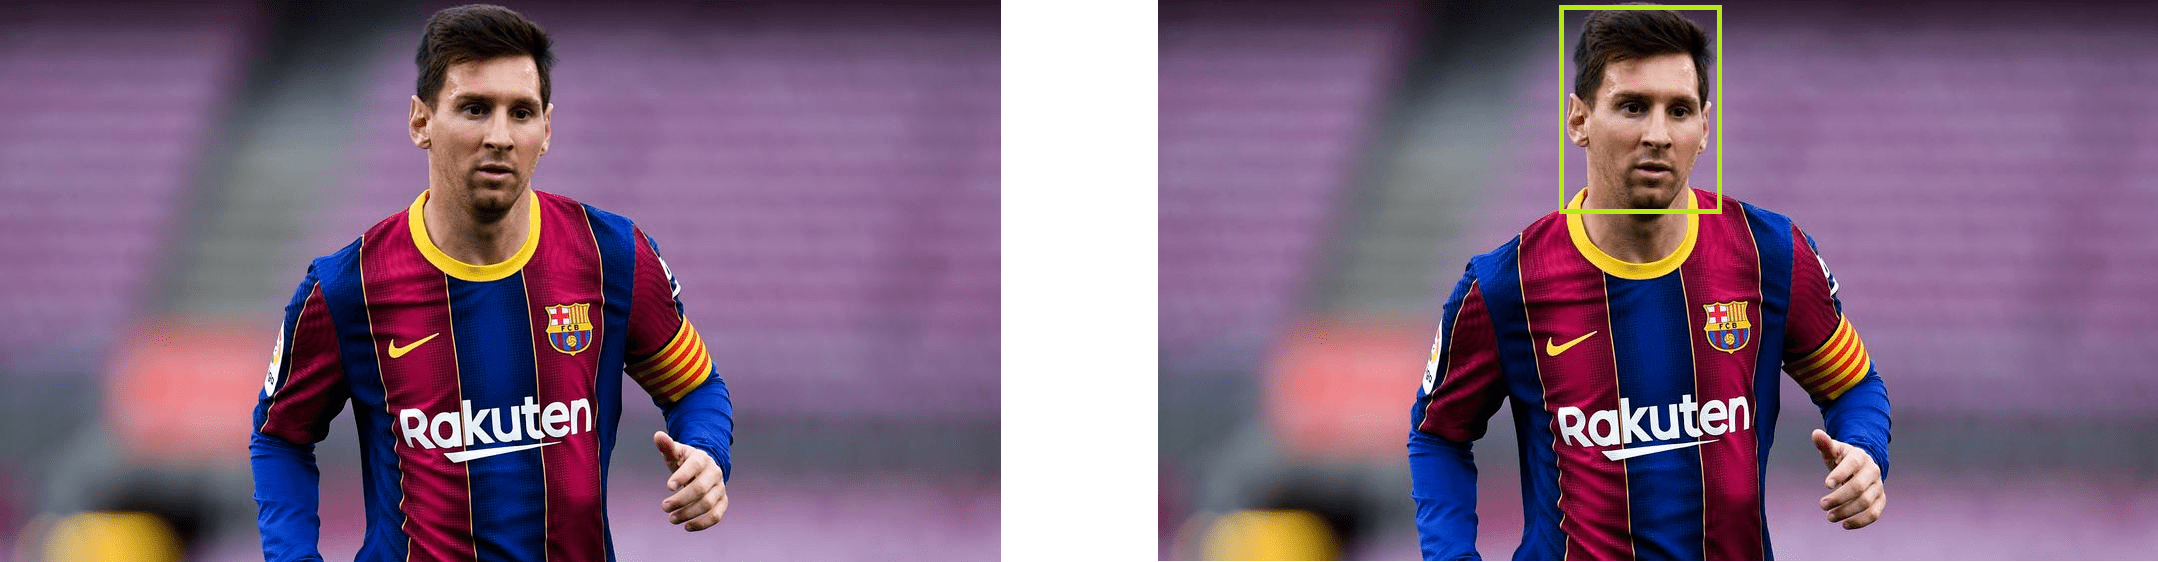
\includegraphics{obrazky-figures/fdexample.png}}
  \label{fdexample}
  \caption{Příklad detekce obličeje}
  \end{center}
\end{figure}

\section{Detekce obličeje}
Detekci obličeje lze rozdělit do několika přístupů, vědecké práce na toto téma se liší a nelze jasně říci zda to či ono dělení je jediné korektní.

Dle \cite{fdReview} existují 2 různé přístupy k hledání tváří v obrázcích, a to \textbf{přístup založený na vlastnostech} (anglicky feature based approach) a \textbf{přístup založený na obrázku} (anglicky image based approach). 
\textbf{Přístup založený na vlastnostech} nepoužívá přímo k detekci obličeje umělou inteligenci a neuronové sítě. Využívá vlastností obličeje jako takového (rysy, pozice očí, uší, obočí\dots).
Naproti tomu \textbf{obrazový přístup} uplatňuje schopnosti neuronových sítí a umělé inteligence k natrénování modelu neuronové sítě a následné přímé detekci pomocí tohoto modelu.

Podle \cite{feature-based-fd-review} lze rozdělit metody detekce obličeje do 4 základních kategorií (viz obrázek \ref{fddeleni}) a 2 zvláštních kategorií (Haarovy vlastnosti a umělá inteligence).

\begin{figure}[H]
  \begin{center}
      \scalebox{0.9}{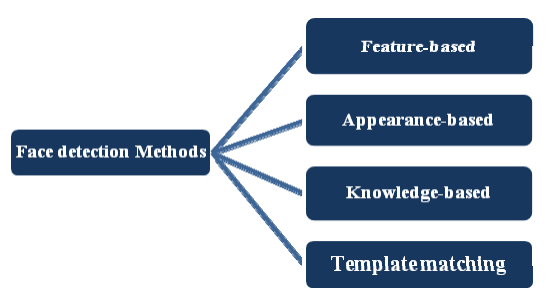
\includegraphics{obrazky-figures/fddeleni.png}}
  \label{fddeleni}
  \caption{Dělení metod detekce obličeje dle \cite{feature-based-fd-review}}
  \end{center}
\end{figure}

Detekce pracující na principu rozpoznávání vlastností v obraze jsou popsány v sekci 
\ref{sekce:detektory_bez_neuronovych_siti}, 
detekce s využitím obrazového přístupu popisuje sekce \ref{sekce:detektory_s_neuronovymi_sitemi}.



\section{Problémy a omezení}
Algoritmy pro detekci obličejů čelí několika výzvám a omezením spojených s ne vždy perfektním zobrazením obličeje v obrázku. Lidské obličeje na fotografiích a obrázcích mohou být částečně zakryté (např. sluneční brýle), mohou být pořízené za nevhodných světelných podmínek (např. zastínění části tváře) nebo mohou nabývat nedostatečné kvality (nízké rozlišení).

Jelikož tedy vstupní obrázek detekce obličeje nemusí být vždy ideální, nemusí být obličej vždy správně detekován.
V této sekci jsou popsány některé problémy \cite{feature-based-fd-review}, které mohou bránit v úspěšné detekci. Minimalizace dopadu těchto jevů na detekci je klíčem k navýšení uspěšnosti detekce. Mezi problémy a omezení (viz obrázek \ref{fdproblems}) pro detekci patří pozice hlavy, zakrytí části/částí obličeje, špatně osvětlená scéna nebo výraz tváře.

\begin{figure}[H]
  \begin{center}
      \scalebox{0.5}{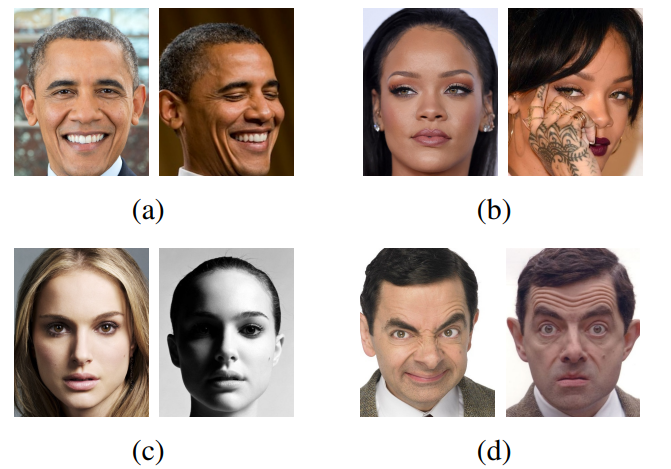
\includegraphics{obrazky-figures/fdproblems.png}}
  \label{fdproblems}
  \caption{Vybráné problémy při detekci obličejů. Převzato z \cite{frReview}. (a) Pozice hlavy; (b)~Zakrytí části obličeje; (c) Špatné světelné podmínky; (d) Výraz tváře}
  \end{center}
\end{figure}

\subsection*{Pozice hlavy}

\subsection*{Výraz tváře}

\subsection*{Orientace obrázku}

\subsection*{Špatné světelné podmínky}

\subsection*{Zakrytí části obličeje}

\subsection*{Nedostatečně výkonná detekce}

\subsection*{Příliš členité pozadí} 

\subsection*{Přílišný počet obličejů v obrázku}

\subsection*{Barva kůže}
zdroj 7 z citace \cite{feature-based-fd-review}

\subsection*{Nízké rozlišení}

\section{Detektory nevyužívající neuronové sítě}
\label{sekce:detektory_bez_neuronovych_siti}



%%%%%%%%%%%%%%%%%%%
%         KaPITOLA
%%%%%%%%%%%%%%%%%%%
\chapter{Neuronové sítě pro detekci obličeje}

\section{Neuronové sítě}

\section{Datasety}

\section{Detektory obličeje}
\label{sekce:detektory_s_neuronovymi_sitemi}

\section{Akcelerace detekce}

\subsection*{Intel Neural Compute Stick 2}





%%%%%%%%%%%%%%%%%%%%%%%%%%%%%%%%%%%%%%%%%%%%%%%%%%%%%%%%%
%       KAPITOLA 4
%%%%%%%%%%%%%%%%%%%%%%%%%%%%%%%%%%%%%%%%%%%%%%%%%%%%%%%%%

\chapter{Implementace algoritmu pro akceleraci detekce obličeje}
\label{kapitola:implementace}
\todo{\blindtext}

\section{Použité nástroje}
\todo{\blindtext}

\section{Trénování neuronové sítě}
\todo{\blindtext}

\section{Detekce obličejů natrénovanou sítí}
\todo{\blindtext}


%%%%%%%%%%%%%%%%%%%%%%%%%%%%%%%%%%%%%%%%%%%%%%%%%%%%%%%%%
%       KAPITOLA 5
%%%%%%%%%%%%%%%%%%%%%%%%%%%%%%%%%%%%%%%%%%%%%%%%%%%%%%%%%

\chapter{Porovnání výkonnosti řešení s existujícími detektory}
\label{kapitola:porovnani_vykonnosti}
\todo{\blindtext}

\section{Postup testování}
\todo{\blindtext}
\begin{figure*}[h]\centering
  \centering
  
\includegraphics[width=\linewidth,height=1.7in]{obrazky-figures/placeholder.pdf}\\[1pt]
  \label{TODO}
  \caption{TODO}
\end{figure*}

\section{Porovnání výsledků}
\todo{\blindtext}

\section{Shrnutí}
\todo{\blindtext}

%%%%%%%%%%%%%%%%%%%%%%%%%%%%%%%%%%%%%%%%%%%%%%%%%%%%%%%%%
%       KAPITOLA 6
%%%%%%%%%%%%%%%%%%%%%%%%%%%%%%%%%%%%%%%%%%%%%%%%%%%%%%%%%
\chapter{Závěr}
\label{kapitola:zaver}
\todo{\Blindtext}